%!TEX root=main.tex

\section{Implémentation et résultats}
\label{section:implementation}

La phase d'implémentation de notre projet ayant été entreprise tardivement, il ne s'agit pas de la plus aboutie et de nombreuses autres pistes de recherche sont encore à explorer. Nous exposons toutefois dans cette section celles que nous avons empruntées ainsi que les résultats obtenus.

\subsection{Implémentation} 
Notre implémentation a été réalisée en Python et se découpe en différents modules et classes.

\begin{itemize}
	
	\item[$\bullet$]\textbf{Module MinHeap} permet de représenter la structure de tas nécessaire à l'exécution de l'algorithme \textsc{DijkstraMinMax}. 
	\item[$\bullet$]\textbf{Module DijkstraMinMax} regroupe toutes les méthodes nécessaires à l'algorithme \textsc{DijkstraMinMax} ainsi que des méthodes pour récupérer les résultats de ce dernier.
	\item[$\bullet$]\textbf{Module GraphGame} comprend :
	\begin{itemize}
		\item[$\star$] \textbf{Classe Graph} pour représenter un graphe ainsi que différentes fonctions pour effectuer des manipulations sur ce dernier.
		\item[$\star$] \textbf{Classe Vertex} pour représenter un sommet du graphe.
		\item[$\star$] \textbf{Classe ReachabilityGame} qui modélise la structure de jeu d'atteignabilité. Elle regroupe les méthodes nécessaires pour calculer le poids d'un chemin, déterminer si un chemin correspond à l'outcome d'un équilibre de Nash ainsi que les différents algorithmes d'exploration testés.
	\end{itemize}
	
	\item[$\bullet$] \textbf{Les modules DijkstraMinMaxTest, ReachabilityGameTest et TestMinHeap} qui nous ont permis de tester nos algorithmes au fur et à mesure de leur implémentation.
	\item[$\bullet$] \textbf{Main} qui permet de tester nos algorithmes sur des graphes générés aléatoirement.
\end{itemize}

Bien que la plupart de nos algorithmes sont utilisables dans des cas plus généraux, nous avons fixé certaines conditions sur les jeux considérés.

\begin{itemize}	
	\item[$\bullet$] Jeux à deux joueurs,
	\item[$\bullet$] Un seul objectif par joueur (ces deux objectifs étant différents), 
	\item[$\bullet$] Le graphe du jeu est un graphe complet (excepté l'arc d'un noeud vers lui-même),
	\item[$\bullet$] La fonction de poids considérées est de la forme $w : E \rightarrow [1,100] \cap \mathbb{N} $.
\end{itemize}

Comme nous l'avons déjà évoqués, plusieurs approches ont été testées afin de trouver un équilibre de Nash pertinent. Nous les expliquons brièvement ci-après.

\subsubsection*{Méthode aléatoire}
De loin la plus naïve, la méthode aléatoire génère de manière aléatoire à partir du sommet initial un certain nombre de chemins (ce nombre est paramétrable) dans le graphe du jeu et ne retient que ceux qui correspondent à l'outcome d'un équilibre de Nash. La longueur de ce chemin est la longueur maximale des chemins à tester. A partir de ce résultat, une méthode a été implémentée afin de ne retenir que l'équilibre le plus pertinent.

\subsubsection*{Breadth-first search}
Nous avons également à notre disposition un algorithme Breadth-first search qui a été un peu modifié. En effet, au lieu de retourner directement le premier objectif rencontré lors du parcours de l'arbre, il est possible de les stocker et de tous les retourner. Nous pouvons ensuite, comme pour la méthode précédente retenir uniquement l'équilibre le plus pertinent. Comme le parcours de tout l'arbre d'exploration peut prendre beaucoup de temps  (complexité exponentielle), il est possible de préciser une limite de temps pour l'exécution de l'algorithme. Une fois cette limite dépassée, ce dernier renvoie tous les équilibres trouvés durant ce laps de temps.

\subsubsection*{Best-first search}

Une implémentation de la méthode d'exploration best-first search a également été mise en \oe uvre. Nous l'avons toutefois amélioré au vu de l'utilisation que nous en faisons. En effet, dans certains cas, il est possible de couper des branches de l'arbre d'exploration:

\begin{itemize}
	\item[$\bullet$] Si le chemin dans le noeud en cours de traitement a atteint la longueur maximale des chemins à tester, il est inutile de pratiquer l'expansion à partir de ce noeud.
	\item[$\bullet$]Si lors de l'expansion d'un noeud, et donc de l'ajout d'un sommet $v_i$ du graphe du jeu au chemin en cours de construction, le noeud  $v_i$ ajouté correspond à un sommet objectif d'un joueur $j$ n'ayant pas encore atteint son objectif, alors on peut appliquer le critère de la propriété~\ref{prop:rechEqpert1}. En effet, si cette propriété n'est pas respectée pour le joueur $j$ alors il ne sert à rien de continuer l'exploration à partir de ce chemin.
\end{itemize}

Comme pour l'approche précédente, une limite sur le temps d'exécution de l'algorithme peut être paramétrée. De plus, n'importe quelle fonction d'évaluation peut être passée en paramètre afin d'ordonner les noeuds dans la frontière. Dans notre cas, après plusieurs tentatives de fonction d'évaluation peu convaincantes, nous avons effectué nos tests à partir de la fonction d'évaluation correspondant à l'algorithme $A^*$ (cf. section~\ref{subsubsection:aStar}).

\subsubsection*{Best-first-search initialisé}

Au lieu de commencer l'exploration à partir du chemin composé uniquement du noeud initial $v_0$, nous avons tenté de guider au mieux le début de la recherche. Pour ce faire nous précédons de la manière suivante: si $o_1$ (resp. $o_2$) est le noeud objectif de $J_1$ (resp. $J_2$) on construit dans un premier temps le chemin le plus court de $v_0$ à $o_1$, si ce chemin n'enfreint pas le critère pour être un équilibre de Nash, alors on lance le best-first search à partir du chemin $v_0 ... o_1$. Si par contre le chemin ainsi constitué enfreint le critère ou si la recherche prend trop temps, on recommence à partir du plus court chemin entre $v_0$ et $o_2$.


%!TEX root=main.tex

\subsection{Résultats}

Nous exposons dans cette section les résultats obtenus sur les quelques tests que nous avons effectués.

\subsubsection*{Tests sur des graphes complets générés aléatoirement}

Afin de tester l'efficacité de l'algorithme $A^*$ que nous avons implémenté, nous avons généré des graphes de manière aléatoire. Pour tout $n \in \mathbb{N}$ tel que $ 5 \leq n \leq 20$, 100 graphes dont les poids sur les arcs sont des entiers entre 1 et 100  ont été créés. L'algorithme a alors été exécuté sur ces instances et nous avons comptabilisé le nombre d'équilibres de Nash qui sont trouvés en permettant un temps de 30 secondes pour chaque exécution de l'algorithme. Les résultats de ces tests\footnote{Tous les tests repris dans ce rapport ont été effectués sur un MacBook Pro, 2,8 GHz Intel Core i5} sont illustrés par le tableau~\ref{tab:premierTest} et par la figure~\ref{fig:premierTest}.
\setlength{\overfullrule}{0pt}

\begin{table}[!ht]
\centering
\caption{Données résultant des tests sur $A^*$}
\label{tab:premierTest}
\begin{tabular}{|l||c|c|c|c|}
	
\hline 
Nombre  & EN & EN & Temps total & Temps moyen  \\ 
de sommets & trouvés & manqués & d'exécution (s) & pour trouver un EN(s) \\ 

\hline 
\hline
5                                                                                 & 100                                                   & 0                                                     & 0,4                                                                    & 0,004                                                                          \\ \cline{1-5}
6                                                                                 & 100                                                   & 0                                                     & 2,37                                                                   & 0,0237                                                                         \\ \cline{1-5}
7                                                                                 & 99                                                    & 1                                                     & 32,45                                                                  & 0,0247                                                                        \\ \cline{1-5}
8                                                                                 & 98                                                    & 2                                                     & 63,08                                                                  & 0,0314                                                                         \\ \cline{1-5}
9                                                                                 & 100                                                   & 0                                                     & 19,76                                                                  & 0,1976                                                                        \\ \cline{1-5}
10                                                                                & 99                                                    & 1                                                     & 46,22                                                                  & 0,1638                                                                        \\ \cline{1-5}
11                                                                                & 95                                                    & 5                                                     & 158,19                                                                 & 0,0862                                                                        \\ \cline{1-5}
12                                                                                & 99                                                    & 1                                                     & 33,86                                                                  & 0,039                                                                         \\ \cline{1-5}
13                                                                                & 98                                                    & 2                                                     & 135,71                                                                 & 0,7726                                                                        \\ \cline{1-5}
14                                                                                & 93                                                    & 7                                                     & 243,86                                                                 & 0,3641                                                                        \\ \cline{1-5}
15                                                                                & 98                                                    & 2                                                     & 80,08                                                                  & 0,2049                                                                        \\ \cline{1-5}
16                                                                                & 96                                                    & 4                                                     & 144,58                                                                 & 0,256                                                                         \\ \cline{1-5}
17                                                                                & 94                                                    & 6                                                     & 248,38                                                                 & 0,7274                                                                        \\ \cline{1-5}
18                                                                                & 93                                                    & 7                                                     & 258,74                                                                 & 0,5241                                                                        \\ \cline{1-5}
19                                                                                & 95                                                    & 5                                                     & 298,07                                                                 & 1,5586                                                                        \\ \cline{1-5}
20                                                                                & 92                                                    & 8                                                     & 331,21                                                                 & 0,9914                                                                        \\ \cline{1-5}
\end{tabular}
\end{table}
\setlength{\overfullrule}{10pt}

\begin{figure}[!ht]  
	\centering
      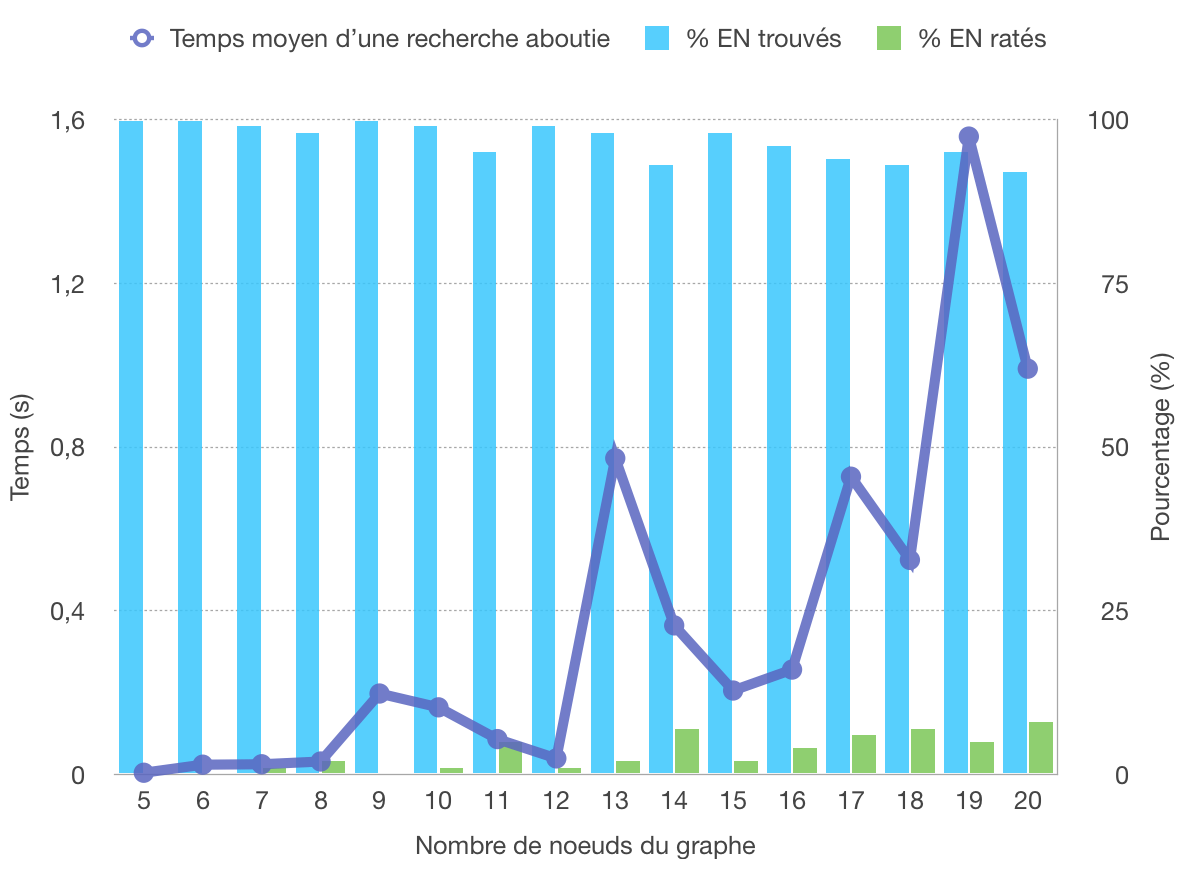
\includegraphics[scale = 0.6]{test_projet/premierTest30.png}
		\caption{Graphique illustrant les résultats des tests sur $A^*$}
		\label{fig:premierTest}
\end{figure}

\FloatBarrier

\subsubsection*{Tests sur des graphes non complets}

Bien que notre objectif était de tester nos algorithmes sur des graphes complets, nous les avons également essayé sur les quelques exemples qui jalonnent notre travail. \\

\noindent \textbf{Premier exemple}

Commençons par nous intéresser par l'exemple~\ref{ex:graphePond} de la page~\pageref{ex:graphePond}. Les résultats retournés en appliquant la méthode aléatoire et l'algorithme $A^*$ sont les suivants:

\begin{code}

A_star : [v1, v2, v3, v0]
Est un EN?  True
Information sur l'outcome : 
Cout pour chaque joueur:  {1: 2, 2: 3}
Joueurs ayant atteint leur objectif  [1, 2]

Random :  [v1, v0, v1, v2, v3, v0, v1, v2,
v4, v3, v4, v2, v3, v4, v3, v0, v1, v0, v1,
v0, v1, v2, v3, v0, v1, v2, v3]
Est un EN?  True
Information sur l'outcome :
Cout pour chaque joueur:  {1: 4, 2: 1}
Joueurs ayant atteint leur objectif  [1, 2]

\end{code}


Nous remarquons que pour les deux outcomes trouvés les deux joueurs atteignent leur objectif et que la somme de leur coût est de 5. Ils sont donc équivalent du point de vue de notre test de pertinence. De plus, si la méthode random est lancée une nouvelle fois, le même outcome que pour l'algorithme $A^*$ est retourné. \\

\noindent \textbf{Deuxième exemple}

Pour l'exemple illustrés dans la section~\ref{subsection:defEqPert} les résultats sont ceux repris ci-dessous.
\begin{code}
A_star : [v0, v2, v0, v1, v3]
Est un EN?  True
Information sur l'outcome : 
Cout pour chaque joueur:  {1: 4, 2: 1}
Joueurs ayant atteint leur objectif  [1, 2]

Random :[v0, v2, v0, v1, v3, v1, v3,
v1, v3, v1, v0, v1]
Information sur l'outcome :
Cout pour chaque joueur:  {1: 4, 2: 1}
Joueurs ayant atteint leur objectif  [1, 2]

\end{code}

Les deux méthodes mènent au même résultat qui est de surcroît le résultat auquel nous nous attendions. \\

\noindent \textbf{Troisième exemple}

Enfin, à partir de l'arène définie dans l'exemple~\ref{ex:dernierExemple} de la page~\pageref{ex:dernierExemple}, on définit $Goal_1 = \{ v_6 \}$ et $Goal_2 = \{ v_0 \}$.

\begin{figure}[ht!]
	\centering

	\begin{tikzpicture}

		\node[nC] (v7) at (0,0){$v_{7}$};
		\node[nR] (v6) at (2,0){$v_{6}$};
		\node[nC] (v5) at (4,0){$v_{5}$};
		\node[nR] (v4) at (6,0){$v_{4}$};
		\node[nC] (v2) at (8,0){$v_{2}$};
		\node[nC] (v0) at (10,0){$v_{0}$};
		\node[nR]  (v1) at (8,2){$v_{1}$};
		\node[nR] (v3) at (8,-2){$v_{3}$};

		\draw[->,>=latex] (v7) to [bend right] node[midway,above]{$1$} (v6);
		\draw[->,>=latex] (v6) to [bend right] node[midway,above]{$1$} (v7);
		\draw[->,>=latex] (v5) to node[midway,above]{$1$} (v6);
		\draw[->,>=latex] (v5) to node[midway,above]{$1$} (v4);


		\draw[->,>=latex] (v4) to node[midway,above]{$5$} (v2);
		\draw[->,>=latex] (v4) to node[midway,left]{$1$} (v3);

		\draw[->,>=latex] (v3) to node[midway,below]{$5$} (v0);
		\draw[->,>=latex] (v3) to node[midway,left]{$1$} (v2);

		\draw[->,>=latex] (v2) to node[midway,above]{$1$} (v0);
		\draw[->,>=latex] (v2) to node[midway,left]{$1$} (v1);

		\draw[->,>=latex] (v1) to node[midway,right]{$1$} (v0);

		\draw[->,>=latex] (v0) to [loop right] node[midway,right]{$1$} (v0);
	\end{tikzpicture}
\end{figure}

Voici les résultats obtenus:

\begin{code} 48

A_star : 
[v3, v2, v0, v0, v0, v0, v0, v0, v0, v0, v0,
v0, v0, v0, v0, v0, v0, v0, v0, v0, v0, v0 ,v0, v0,
v0, v0, v0 , v0, v0, v0, v0, v0 ,v0, v0, v0, v0, v0,
v0, v0, v0, v0, v0 , v0, v0, v0, v0, v0, v0, v0, v0]
Est un EN?  True
Information sur l'outcome : 
Cout pour chaque joueur:  {1: inf, 2: 2}
Joueurs ayant atteint leur objectif  [] 2]

Random :
[v3, v2, v0, v0, v0, v0, v0, v0, v0, v0, v0,
v0, v0, v0, v0, v0, v0, v0, v0, v0, v0, v0 ,v0, v0,
v0, v0, v0 , v0, v0, v0, v0, v0 ,v0, v0, v0, v0, v0,
v0, v0, v0, v0, v0 , v0, v0, v0, v0, v0, v0, v0, v0]
Est un EN?  True
Information sur l'outcome :
Cout pour chaque joueur:  {1: inf, 2: 2}
Joueurs ayant atteint leur objectif  [2]

\end{code}


Puisque depuis le noeud $v_0$ la seule action possible est de boucler sur $v_0$ ce comportement est normal. 

Rajoutons des noeuds à ce graphe afin que celui-ci soit un graphe fortement connexe. Afin de ne pas surcharger le graphe, les arcs qui ne possèdent pas d'étiquette sont des arcs de poids $1$.

\begin{figure}[ht!]
	\centering

	\begin{tikzpicture}

		\node[nC] (v7) at (0,0){$v_{7}$};
		\node[nR] (v6) at (2,0){$v_{6}$};
		\node[nC] (v5) at (4,0){$v_{5}$};
		\node[nR] (v4) at (6,0){$v_{4}$};
		\node[nC] (v2) at (8,0){$v_{2}$};
		\node[nC] (v0) at (10,0){$v_{0}$};
		\node[nR]  (v1) at (8,2){$v_{1}$};
		\node[nR] (v3) at (8,-2){$v_{3}$};

		\draw[->,>=latex] (v7) to [bend right]  (v6);
		
		\draw[->,>=latex] (v6) to [bend right]  (v7);
		\draw[->,>=latex] (v6) to [bend right] node[midway,above]{$2$} (v5);
		
		\draw[->,>=latex] (v5) to [bend right]  (v4);
		\draw[->,>=latex] (v5) to [bend right]  (v6);
		

		\draw[->,>=latex] (v4) to [bend right] (v5);
		\draw[->,>=latex] (v4) to node[midway,above]{$5$} (v2);
		\draw[->,>=latex] (v4) to [bend right]  (v3);

		\draw[->,>=latex] (v3) to [bend right] node[midway,below]{$5$} (v0);
		\draw[->,>=latex] (v3) to [bend right] node[midway, right]{$4$}  (v2);
		\draw[->,>=latex] (v3) to [bend right]  (v4);
		
		

		\draw[->,>=latex] (v2) to [bend right]node[midway,above]{$4$} (v0);
		\draw[->,>=latex] (v2) to (v1);
		\draw[->,>=latex] (v2) to [bend right] (v3);
		

		\draw[->,>=latex] (v1) to  (v0);

		\draw[->,>=latex] (v0) to [bend right](v2);
	\end{tikzpicture}
\end{figure}
\FloatBarrier

Les résultats obtenus sont les suivants  :

\begin{code}

A_star : [v3, v4, v5, v6, v5, v4, v3, v0]
Est un EN?  True
Information sur l'outcome : 
Cout pour chaque joueur:  {1: 3, 2: 12}
Joueurs ayant atteint leur objectif  [1, 2]

Random :  [v3, v4, v5, v6, v5, v4, v3, v2, v1, v0,
v2, v3,v0,v2,v1,v0, v2, v0, v2, v1, v0, v2, v3, v4,
v5, v4, v5,v4, v3, v2, v1, v0, v2, v1, v0, v2, v0,
v2, v1, v0, v2, v1, v0, v2, v1, v0, v2, v0,v2, v0,
v2,v3, v2, v3, v2, v1, v0, v2, v1,v0, v2, v0, v2,
v1, v0, v2, v1, v0, v2]
Est un EN?  True
Information sur l'outcome :
Cout pour chaque joueur:  {1: 3, 2: 13}
Joueurs ayant atteint leur objectif  [1, 2]

\end{code}

Le résultat retourné par l'algorithme $A^*$ est meilleur que celui de la méthode aléatoire. En effet, pour le premier la somme des coûts des joueurs est de 15 tandis que pour le second 16. 

\subsubsection*{Comparaison des résultats}

Afin de pouvoir comparer nos différentes méthodes, une série de test est générée. Nous avons exécuté nos tests comme suit : nous générons aléatoirement 100 jeux qui respectent les conditions explicitées dans le section~\ref{section:implementation} et dont le graphe du jeu possède 5 sommets. Ensuite, les quatre méthodes auxquelles nous nous sommes intéressées sont exécutées sur chacun de ces jeux en permettant un temps d'exécution de 30 secondes pour chaque méthode et en générant 100 chemins différents pour la méthode aléatoire. Puisque nous voulons tester l'efficacité du best-first search avec l'utilisation de la fonction d'évaluation de type $A^*$, qui nous semble être l'approche la plus aboutie, chaque résultat obtenu est comparé avec celui de cette méthode. Nous avons alors cinq possibilités, $A^*$ est:
\begin{itemize}
	\item[$\bullet$] meilleur;
	\item[$\bullet$] pire;
	\item[$\bullet$] égal (le même outcome est retourné pour les deux méthodes);
	\item[$\bullet$] équivalent (un outcome différent est retourné pour les deux méthodes, mais le nombre de joueurs ayant atteint leur objectif ainsi que la somme des coûts pour ceux-ci sont égaux);
	\item[$\bullet$] les deux méthodes ont échoués (une méthode échoue si elle n'a pas trouvé d'équilibre de Nash endéans le temps imparti)
\end{itemize}

En plus de cela, le temps nécessaire pour l'exécution des 100 recherches pour chaque méthode est calculé.\\
Les résultats de ces tests sont repris dans le tableau~\ref{tab:compMet} et à la figure~\ref{fromages}.

\begin{table}[!ht]
	\caption{Comparaison des différentes méthodes}
	\label{tab:compMet}
	\begin{tabular}{|l||c|c|c|}
		\hline
		Méthode & EN trouvés & EN manqués & Temps moyen\\
				&			 &			 & de recherche (s)\\
		\hline
		\hline
		
		$A^*$ & 100 & 0 & 0,0028\\
		\hline
		Méthode aléatoire & 97 & 3 & 1,135\\
		\hline
		Best-first search initialisé & 95 & 5 & 6,6105 \\
		\hline
		Breadth-first search & 100 & 0 & 0,0054\\
		\hline
	\end{tabular}
	
\end{table}
\setlength{\overfullrule}{0pt}

\begin{figure}     
      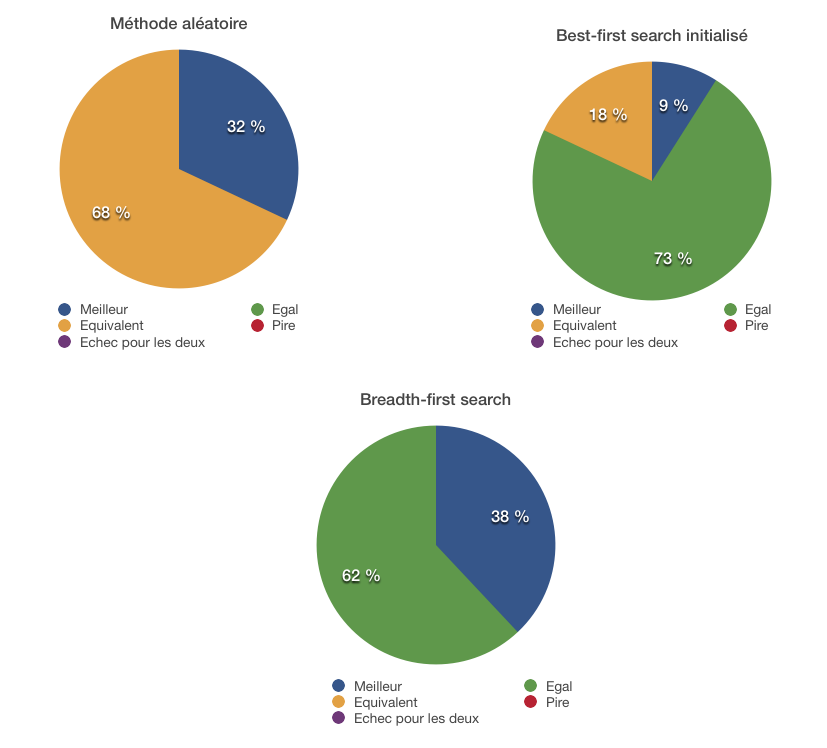
\includegraphics[scale = 0.5]{test_projet/result_method}
		\caption{Comparaison d'$A^*$ avec les trois autres méthodes}
		\label{fromages}

\end{figure}
\setlength{\overfullrule}{10pt}
\FloatBarrier



Bien que peu de tests permettant de comparer les différentes approches aient été effectués, nous pouvons toutefois tirer quelques conclusions:

\begin{itemize}
	\item[$\bullet$] La méthode best-first search en utilisant la fonction  d'évaluation $A^*$ est celle la plus aboutie. En effet, au vu des résultats sur les graphes complets, un équilibre est trouvé en moins de 30 secondes dans plus de 90\% des tests. De plus, si l'on regarde les tests de comparaison avec les autres méthodes, cette méthode est meilleure aussi bien au point de vue du temps nécessaire pour trouver un équilibre de Nash, ainsi que sur la qualité de celui-ci. 
	\item[$\bullet$] La méthode aléatoire trouve généralement un équilibre de Nash mais rien ne garantit l'optimalité de celui-ci. De plus, dans certains cas, elle peut ne retourner aucun résultat.	
	\item[$\bullet$] La méthode de best-first search initialisé, qui est une des premières approches que nous avons testée, est celle qui nous garantissait les meilleurs résultats avant que nous ne changions la fonction d'évaluation de notre best-first search. Elle comporte divers inconvénients. Puisque l'on teste l'initialisation du chemin jusqu'au premier noeud initial, que l'on attend un certain laps de temps puis seulement que l'on relance la recherche, cette approche est peut s'avérer coûteuse en temps. De plus, elle ne trouve pas toujours d'équilibre de Nash dans le temps imparti.
	\item[$\bullet$] Si la méthode breadth-first search est utilisée en renvoyant le premier équilibre trouvé alors, puisqu'elle parcourt les chemins par taille croissante, cette recherche n'est pas optimale. En effet, il se peut qu'un chemin d'une plus longue taille mais de poids moindre soit préférable à un chemin plus court. Il en va de même, si on récupère tous les équilibres trouvés pendant un certain laps de temps. De plus, pour cette dernière procédure, le temps d'exécution est toujours égal au temps d'exécution permis.
\end{itemize}
$ $\\
\textbf{Remarquons que les temps de calcul repris dans les tableaux~\refrangeconj{tab:premierTest}{tab:compMet} sont les temps nécessaires pour que les algorithmes retournent une solution et non les temps CPU. Ces données sont calculées afin de nous faire une idée sur l'ordre de grandeur du temps nécessaire à l'exécution de nos méthodes. Toutefois, pour une étude plus fine, la réalisation de tests tenant compte du temps CPU sertait plus pertinente.}





	